\section{Robustness of the Statistical Comparisons}
\label{sec:rob}

\subsection*{Statistical setup}

We assess whether the reported performance differences are statistically reliable and survive choices about how significance is decided. For each dataset and headline metric (F1, nDCG@10, MAP, MRR) we run the two-sided paired t-test across the ten seeds ($df = 9$) for \textbf{every pair of the eight models} --- 28 comparisons per dataset $\times$ metric, 224 in total. Because all models share the same per-seed test splits, the comparisons are naturally paired and the t-statistic preserves direction (the higher-mean model appears on the left of each inequality).

With 28 simultaneous tests per family, uncorrected p-values would overstate evidence, so we apply multiplicity correction as the primary analysis: \textbf{Holm-Bonferroni step-down adjustment} (\citep{holm1979simple}), which controls the family-wise error rate while remaining strictly more powerful than plain Bonferroni. As a stress test we additionally report \textbf{Bonferroni correction} (threshold $\alpha$/28 $\approx$ 0.0018 at $\alpha = 0.05$). Throughout, ``significant'' means corrected $p < \alpha$, and a pair is said to be \textbf{lost} when it is significant under Holm but not under Bonferroni.

\subsection{Multiplicity correction: Holm vs Bonferroni}
\label{sec:rob-corr}

At $\alpha = 0.05$ the raw analysis finds 28/28 comparisons significant on both datasets for F1, nDCG@10 and MAP, and 27/28 for MRR; the single non-significant raw comparison is \textbf{BM25 vs TF-IDF} under MRR ($p = 0.3351$ / 0.1554 on FIRE-AgentIR-2026 / FIRE-CrossLingIR-2026), a near-tie that is never significant at any threshold we consider.

\textbf{Holm-Bonferroni leaves every raw-significant comparison intact:} the corrected counts are identical to the raw counts on every metric and dataset (F1, nDCG@10, MAP: 28/28; MRR: 27/28). Holm applies its smallest multipliers (1--2) to the largest raw p-values, so marginal comparisons (raw p $\approx$ 0.002--0.046, e.g. MRR on AgentIR: $p = 0.0236$ $\rightarrow$ 0.0472) still pass, while all remaining comparisons have raw $p \leq 0.001$. Under the harsher Bonferroni correction, however, those same marginal pairs drop out. \Cref{tab:corr-counts} summarizes the counts; the eight lost pair-instances are enumerated in \Cref{tab:lost-pairs}.

\begin{table*}[tb]
\setlength{\tabcolsep}{3pt}
\footnotesize
\caption{Significant pairwise comparisons (of 28) at $\alpha = 0.05$ under each correction, per dataset $\times$ metric. ``lost'' = significant under Holm but not under Bonferroni.}
\label{tab:corr-counts}
\centering
\begin{tabular}{lccccc}
\toprule
Metric & Dataset & raw & Holm & Bonferroni & lost \\
\midrule
F1 & FIRE-AgentIR-2026 & 28/28 & 28/28 & 28/28 & 0 \\
F1 & FIRE-CrossLingIR-2026 & 28/28 & 28/28 & 28/28 & 0 \\
nDCG@10 & FIRE-AgentIR-2026 & 28/28 & 28/28 & 26/28 & 2 \\
nDCG@10 & FIRE-CrossLingIR-2026 & 28/28 & 28/28 & 27/28 & 1 \\
MAP & FIRE-AgentIR-2026 & 28/28 & 28/28 & 26/28 & 2 \\
MAP & FIRE-CrossLingIR-2026 & 28/28 & 28/28 & 27/28 & 1 \\
MRR & FIRE-AgentIR-2026 & 27/28 & 27/28 & 26/28 & 1 \\
MRR & FIRE-CrossLingIR-2026 & 27/28 & 27/28 & 26/28 & 1 \\
\bottomrule
\end{tabular}
\end{table*}

The eight lost pair-instances belong to exactly two comparison families --- \textbf{BM25 vs TF-IDF} (the two classical baselines) and \textbf{MEIRA-no-decay vs ColBERT-like} (the strongest ablation variant against the strongest neural baseline) --- and never involve MEIRA-full:

\begin{table*}[tb]
\setlength{\tabcolsep}{3pt}
\footnotesize
\caption{The eight pair-instances that are significant under Holm but not under Bonferroni at $\alpha = 0.05$.}
\label{tab:lost-pairs}
\centering
\begin{tabular}{lcccccc}
\toprule
Metric & Dataset & Pair & raw p & Holm p & Bonferroni p & t \\
\midrule
nDCG@10 & FIRE-AgentIR-2026 & BM25 > TF-IDF & 0.0105 & 0.0141 & 0.2927 & 3.22 \\
nDCG@10 & FIRE-AgentIR-2026 & MEIRA-no-decay > ColBERT-like & 0.0071 & 0.0141 & 0.1979 & 3.47 \\
nDCG@10 & FIRE-CrossLingIR-2026 & BM25 > TF-IDF & 0.0458 & 0.0458 & 1.0000 & 2.32 \\
MAP & FIRE-AgentIR-2026 & BM25 > TF-IDF & 0.0034 & 0.0068 & 0.0946 & 3.95 \\
MAP & FIRE-AgentIR-2026 & MEIRA-no-decay > ColBERT-like & 0.0044 & 0.0068 & 0.1241 & 3.77 \\
MAP & FIRE-CrossLingIR-2026 & BM25 > TF-IDF & 0.0247 & 0.0247 & 0.6907 & 2.69 \\
MRR & FIRE-AgentIR-2026 & MEIRA-no-decay > ColBERT-like & 0.0236 & 0.0472 & 0.6605 & 2.72 \\
MRR & FIRE-CrossLingIR-2026 & MEIRA-no-decay > ColBERT-like & 0.0023 & 0.0045 & 0.0635 & 4.21 \\
\bottomrule
\end{tabular}
\end{table*}

The key observation is what is \textbf{not} in \Cref{tab:lost-pairs}: every comparison involving \textbf{MEIRA-full --- including vs the best baseline ColBERT-like --- remains significant at $p < 0.0001$ even after Bonferroni correction} on every metric and dataset. The headline superiority claim therefore does not depend on which correction is chosen.

\Cref{fig:ordering} tracks every model's rank across the four ranking-quality metrics and flags the models involved in adjacencies that remain non-significant after Holm correction (dashed lines) --- the only places where the reported ordering could flip. MEIRA-full holds rank 1 on both datasets and every metric, and BM25 vs TF-IDF is the sole fragile comparison.

\begin{figure*}[tb]
\centering
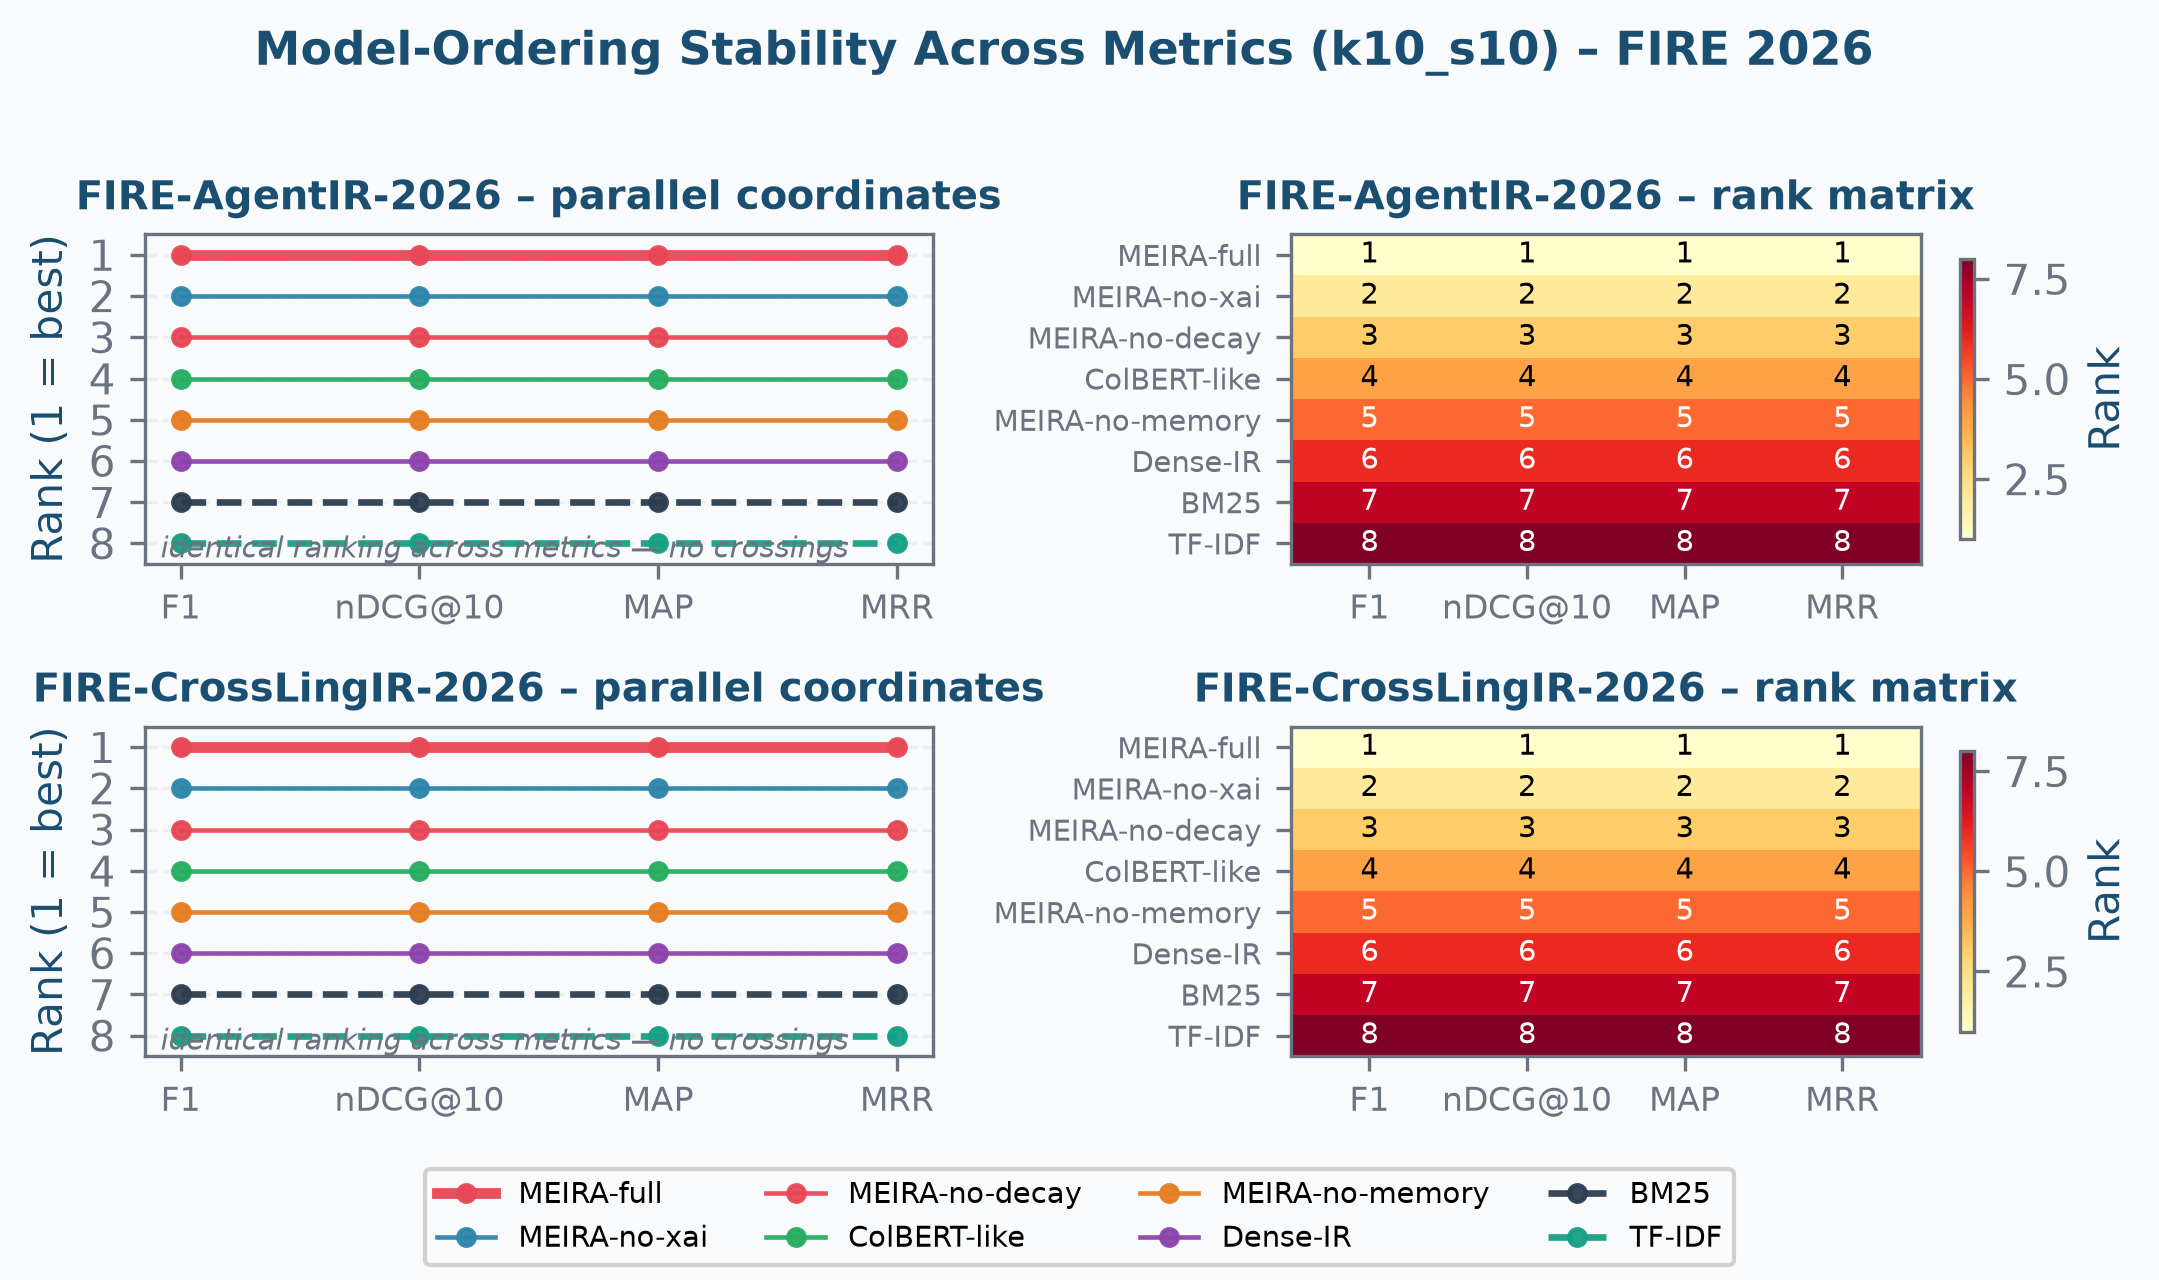
\includegraphics[width=0.94\textwidth]{../figures/k10_s10/ord1_ordering_stability_holm.png}
\caption{Parallel coordinates of per-metric model ranks (left) and rank matrix (right) on both datasets; dashed lines mark models involved in Holm-non-significant adjacencies.}
\label{fig:ordering}
\end{figure*}

\subsection{Threshold sensitivity: $\alpha \in \{0.01, 0.05, 0.10\}$}
\label{sec:rob-alpha}

To verify the verdicts are not an artifact of the $\alpha = 0.05$ convention, we re-evaluate every comparison at $\alpha = 0.01$ and $\alpha = 0.10$ (p-values are threshold-independent; only verdicts move). Two conclusions hold:

\textbf{F1 is invariant.} All 28 comparisons are significant under every correction at every $\alpha$ on both datasets: the F1 leaderboard is completely insensitive to both the correction and the threshold.

\textbf{Holm is nearly threshold-stable.} Across the 24 dataset $\times$ metric $\times$ threshold conditions, Holm's adjustment flips exactly \textbf{one} raw-significant verdict: at $\alpha = 0.01$, MEIRA-no-decay > ColBERT-like on AgentIR (raw $p = 0.0071$ < 0.01, Holm $p = 0.0141$ > 0.01) drops out. The other $\alpha = 0.01$ reductions are raw-threshold effects (raw p-values 0.0105--0.0458 already exceed 0.01); the MRR non-significance of BM25 vs TF-IDF is inherited by Holm at every threshold.

Bonferroni is where the threshold binds: at $\alpha = 0.01$ it drops more comparisons (e.g. MAP on FIRE-CrossLingIR-2026: 24/28, plus a few CrossLing micro-gaps joining the fragile families), while at $\alpha = 0.10$ it \emph{recovers} exactly two of the eight $\alpha = 0.05$ losses (MRR no-decay > ColBERT-like on CrossLingIR, $p = 0.0635$; MAP BM25 > TF-IDF on AgentIR, $p = 0.0946$). In total, 14 pair-instances across the sweep are \textbf{$\alpha$-sensitive}, and \textbf{none of them involves MEIRA-full}. The unstable comparisons are again the two fragile families plus a few tight CrossLing ablation-tier gaps; no ordering \emph{direction} ever flips, only the verdict.

% ==== DRAFTING METADATA (was: 5.3 Defensible claims) ====

%
% 1. **MEIRA-full is robustly superior.** Its advantage over every other
%    model is significant at p < 0.0001 on the headline metrics under both
%    Holm and Bonferroni correction and at all α ∈ {0.01, 0.05, 0.10}; no
%    comparison involving MEIRA-full is ever lost. This claim is safe to make
%    unconditionally.
% 2. **The ablation ladder is reliable under Holm.** All variant-vs-variant
%    differences survive Holm correction at α = 0.05; under the stricter
%    Bonferroni only the no-decay/ColBERT boundary (Section 5.1) and a few CrossLing
%    micro-gaps at α = 0.01 (Section 5.2) are affected.
% 3. **BM25 > TF-IDF is fragile and should be phrased as a tendency, not a
%    claim.** It is significant under F1 (p < 0.0001 on AgentIR, p = 0.0003
%    on CrossLingIR) and marginal under nDCG@10/MAP (Holm p =
%    0.0068–0.0458), non-significant under MRR, and lost under Bonferroni
%    wherever it passes at α = 0.05. Its direction never
%    flips, but the evidence for separating the two classical baselines is the
%    weakest in the leaderboard.
% 4. **MEIRA without temporal decay vs the best neural baseline is the one
%    place to hedge.** MEIRA-no-decay > ColBERT-like is significant under
%    Holm on both datasets but is lost under Bonferroni on four of its eight
%    significant occurrences; claims that no-decay MEIRA "beats the best
%    neural baseline" should cite the Holm-corrected (not raw) p-values and
%    note the Bonferroni sensitivity.
%
% *These conclusions were produced from the simulated harness; see the status
% note at the top. Full per-pair data: `results/k10_s10/correction_comparison.md`
% and `results/k10_s10/alpha_sweep.md` (machine-readable: `.json` twins;
% figures: `corr1_correction_comparison.png`, `sweep1_alpha_counts.png`).*
%
% ---
